% http://steventhornton.ca/blog/markov-chains-in-latex.html
\documentclass{standalone}
\usepackage{tikz}
\usetikzlibrary{automata, positioning}

\newcommand{\createNode}[6]{
  \node[
    state,
    text=#5,
    fill=#6
  ] at (#3,#4)(#1){#2};
}
\newcommand{\createEdge}[5]{
  \draw[
    every loop,
    bend right,
    auto=right,
    text=#4,
    fill=#5
  ] (#1) edge node{#3} (#2);  
}

\begin{document}
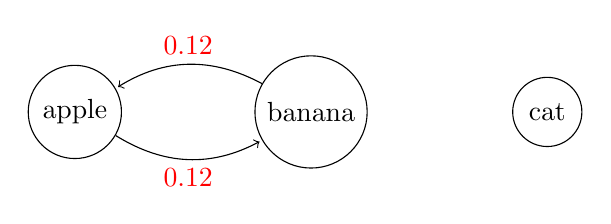
\begin{tikzpicture}
  % python generate 
  \createNode{a}{apple}{0}{0}{black}{white}
  \createNode{b}{banana}{3}{0}{black}{white}
  \createNode{c}{cat}{6}{0}{black}{white}
  \createEdge{a}{b}{0.12}{red}{black}
  \createEdge{b}{a}{0.12}{red}{black}
  
\end{tikzpicture}
\end{document}

